\documentclass[11pt]{article}

\newcommand{\cnum}{CS M146}
\newcommand{\ced}{Winter 2019}
\newcommand{\ctitle}[3]{\title{\vspace{-0.5in}\cnum, \ced\\Problem Set #1: #2\\Due #3}}
\usepackage{enumitem}
\newcommand{\solution}[1]{{{\color{blue}{\bf Solution:} {#1}}}}
\usepackage[usenames,dvipsnames,svgnames,table,hyperref]{xcolor}
\usepackage{graphicx}
\usepackage[tbtags]{amsmath}
\usepackage[hang, small,labelfont=bf,up]{caption} % Custom captions under/above floats in tables or figures
\usepackage{booktabs} % Horizontal rules in tables


\renewcommand*{\theenumi}{\alph{enumi}}
\renewcommand*\labelenumi{(\theenumi)}
\renewcommand*{\theenumii}{\roman{enumii}}
\renewcommand*\labelenumii{\theenumii.}


\begin{document}
\ctitle{2}{Perceptron and Regression}{Feb 12, 2019}
\author{Tian Ye \\ \small{Collaborator: Derek Chu}}
\maketitle

\newpage

\section{Perceptron}
\begin{enumerate}
\item 

\solution{
We start with the truth table for the OR function:
\begin{displaymath}
\begin{array}{|c c|c|}
x_1 & x_2 & x_1 \lor x_2\\ 
\hline  
0 & 0 & 0\\
1 & 0 & 1\\
1 & 1 & 1\\
0 & 1 & 1\\
\end{array}
\end{displaymath}
From the table we can now start solving for $w_1$ and $w_2$:

\begin{align}
w_1*0 + w_2*0 - b &< 0 \\
w_1*1 + w_2*0 - b &> 0 \\
w_1*1 + w_2*1 - b &> 0 \\
w_1*0 + w_2*1 - b &> 0
\end{align}

From this we yield $b > 0$, and we can create a valid perceptron, such as by using $w_1 = 2$, $w_2 = 2$, and $b = 1$. \\
We can show that the perceptron is not unique, by creating a second perceptron using the following parameters: \\
$w_1 = 2$, $w_2 = 2$, and $b = 1.5$.
}
\vspace{1cm}

\item
\solution{
We start with the truth table for the XOR function:
\begin{displaymath}
\begin{array}{|c c|c|}
x_1 & x_2 & x_1 \oplus x_2\\ 
\hline  
0 & 0 & 0\\
1 & 0 & 1\\
1 & 1 & 0\\
0 & 1 & 1\\
\end{array}
\end{displaymath}
From the table we can now start solving for $w_1$ and $w_2$:

\begin{align}
w_1*0 + w_2*0 - b &< 0 \\
w_1*1 + w_2*0 - b &> 0 \\
w_1*1 + w_2*1 - b &< 0 \\
w_1*0 + w_2*1 - b &> 0
\end{align}

From this we yield $b > 0$, and we can see that there cannot be a valid perceptron as when we combine equations 6 and 8 we yield \\
$w_1*0 + w_2*1 - 2b > 0$, yet equation 7 states that $w_1*1 + w_2*1 - b < 0$. Since $b > 0$, we have a contradiction. Therefore there does not exist a perceptron.
}
\end{enumerate}
\newpage

\section{Logistic Regression}
\begin{enumerate}
\item

\solution{
\begin{align}
J(\theta) &= -\sum_{n=1}^{N}[y_n \log (\sigma(\theta^T x_n)) + (1-y_n)\log(1-\sigma(\theta^T x_n))] \\
\tfrac{\partial J(\theta)}{\partial \theta_i} &= -\sum_{n=1}^{N}\bigg[\tfrac{y_n(\sigma(\theta^T x_n))(1-\sigma(\theta^T x_n))x_{n,i}}{\sigma(\theta^T x_n)}-\tfrac{(1-y_n)(\sigma(\theta^T x_n))(1-\sigma(\theta^T x_n))x_{n,i}}{(1-\sigma(\theta^T x_n))}\bigg] \\
\tfrac{\partial J(\theta)}{\partial \theta_i} &= -\sum_{n=1}^{N} [y_n(1-\sigma(\theta^T x_n))-(1-y_n)(\sigma(\theta^T x_n))]x_{n,i} \\
\tfrac{\partial J(\theta)}{\partial \theta_i} &= -\sum_{n=1}^{N} [y_n-\sigma(\theta^T x_n)]x_{n,i}
\end{align}
Where $x_{n, i}$ is the nth row, ith column.
}
\vspace{1cm}

\item
\solution{
\begin{align}
\tfrac{\partial^2 J}{\partial \theta_i \partial \theta_k} &=\sum_{n=1}^{N} x_{n,i}(\sigma(\theta^T x_n)) (1-\sigma(\theta^T x_n))(\tfrac{\partial }{\partial \theta_k}\theta^T x_n) \\
\tfrac{\partial^2 J}{\partial \theta_i \partial \theta_k} &=\sum_{n=1}^{N} x_{n,i}x_{n,k}(\sigma(\theta^T x_n)) (1-\sigma(\theta^T x_n)) \\
\tfrac{\partial^2 J}{\partial \theta_i \partial \theta_k} &=\sum_{n=1}^{N} x_{n,i}x_{n,k}(h_\theta(x_n))(1-h_\theta(x_n)) 
\end{align}
This is a valid formula for calculating the Hessian as the Hessian is given by $H = \sum_{n=1}^{N} (h_\theta(x_n))(1-h_\theta(x_n))x_n x_n^T$ and if we expand $x_{n,i}x_{n,k}$, then we get that the $H_{i,k}$ element is $x_{n,i}\bullet x_{n,k}$.
}
\newpage

\item
\solution{
\begin{align}
z^THz &= \sum_{i,k}z_i z_k H_{i,k} \geq 0 \\
z^THz &= \sum_{i,k} \sum_{n=1}^{N} z_i z_k H_{i,k} x_{n,i}x_{n,k}(h_\theta(x_n))(1-h_\theta(x_n))
\end{align}
Since $h_\theta(x_n) = \sigma(\theta^Tx_n) = (1+e^{-\theta^T x_n})^-1$, $h_\theta(x_n) > 0$. Furthermore, since $h_\theta(x_n) < 1$, $1-h_\theta(x_n) > 0$ as well. We can then remove those two components from Equation 17 as they are always positive:
\begin{align}
z^THz &= z^T \sum_{n=1}^{N} x_n x_n^T z \\
z^THz &= z^T \sum_{n=1}^{N} XX^T z \\
\end{align}
Where $X$ is the full matrix. Therefore $(X^Tz)^T(X^Tz) > 0$.
}
\end{enumerate}
\newpage

\section{Locally Weighted Linear Regression}
\begin{enumerate}
\item
\solution{
\begin{align}
\tfrac{\partial J}{\partial \theta_0} &= \sum_{n=1}^{N} 2w_n(\theta_0 + \theta_1 x_{n,1}-y_n)\\
\tfrac{\partial J}{\partial \theta_1} &= \sum_{n=1}^{N} 2w_nx_{n,1}(\theta_0 + \theta_1 x_{n,1}-y_n)
\end{align}
\vspace{1cm}

\item
\solution{
\begin{align}
\sum_{n=1}^{N} 2w_n(\theta_0 + \theta_1 x_{n,1}-y_n) &= 0 \\
\theta_0 = -\frac{\sum_{n=1}^{N}w_n(\theta_1 x_{n,1}-y_n)}{\sum_{n=1}^{N}w_n}
\end{align}
\vspace{.5cm}
\begin{align}
\sum_{n=1}^{N} 2w_nx_{n,1}(\theta_0 + \theta_1 x_{n,1}-y_n) &= 0 \\
\theta_1=\frac{\sum_{n=1}^{N}w_nx_{n,1}(\theta_1 x_{n,1}-y_n)}{\sum_{n=1}^{N}w_nx_{n,1}^2}
\end{align}
}
\newpage
\item
\solution
{
\begin{align}
X\theta - y &= 
\begin{bmatrix}
\theta_0 + \theta_1x_{1,1}-y_1 \\
\theta_0 + \theta_1x_{2,1}-y_2 \\
\vdots \\
\theta_0 + \theta_1x_{N,1}-y_N \\
\end{bmatrix}\\
(X\theta - y)^T &=
\begin{bmatrix}
\theta_0 + \theta_1x_{1,1}-y_1 \hdots \theta_0 + \theta_1x_{N,1}-y_N \\
\end{bmatrix} \\
W &= 
\begin{bmatrix}
w_1 & 0 & \hdots & \hdots & 0 \\
0 & w_2 &&& \vdots \\
\vdots && \ddots && \vdots\\
\vdots &&& w_{N-1}& 0\\
0 & \hdots & \hdots &0 &  w_N\\
\end{bmatrix} \\
(X\theta - y)^TW &=
\begin{bmatrix}
w_1(\theta_0 + \theta_1x_{1,1}-y_1) \hdots w_N(\theta_0 + \theta_1x_{N,1}-y_N) \\
\end{bmatrix} \\
(X\theta - y)^TW(X\theta - y) &=
\begin{bmatrix}
w_1(\theta_0 + \theta_1x_{1,1}-y_1)^2 \hdots w_N(\theta_0 + \theta_1x_{N,1}-y_N)^2 \\
\end{bmatrix} \\
(X\theta - y)^TW(X\theta - y) &=  \sum_{n=1}^{N} w_n(\theta_0 + \theta_1 x_{n,1}-y_n)^2
\end{align}
}
}
\end{enumerate}
\newpage

\section{Implementation: Polynomial Regression}
\begin{enumerate}
\item
\solution{
\begin{figure}[!htbp]
    \centering
    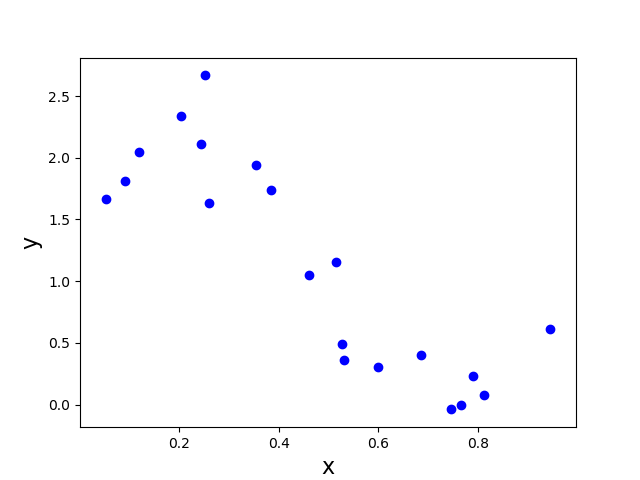
\includegraphics[width=3in]{4atrain.png}
    \caption{Training Data}
\end{figure}
\begin{figure}[!htbp]
    \centering
    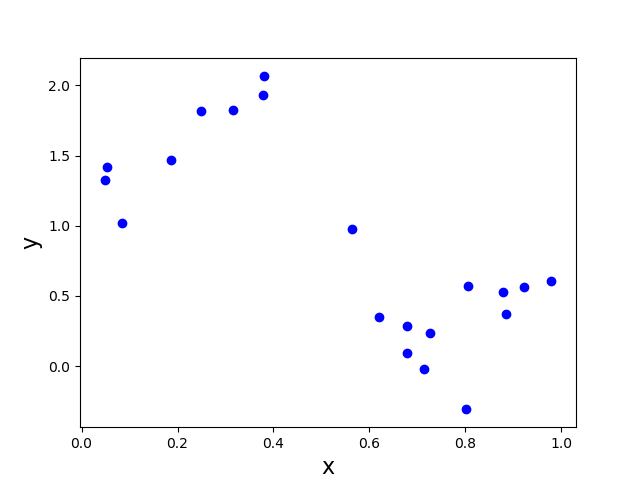
\includegraphics[width=3in]{4atest.png}
    \caption{Test Data}
\end{figure} \\
Viewing both graphs above, we can see that they are as a whole appear to be relatively sinusoidal. However, since the central portion of both graphs are relatively linear, linear regression would be feasible; however, higher order functions should be used for higher accuracy.
}
\newpage

\item
\solution{
Complete.
}
\item
\solution{
Complete.
}

\item
\solution{
\begin{table}[!htbp]
\centering
\scalebox{0.8}{
\begin{tabular}{lllll}
\toprule
\cmidrule{1-5}
Step Size & Coefficients & No. of Iterations & Cost & Time \\
\midrule
$10^{-4}$ &  [ 1.91573585 -1.74358989] & 10,000 & 5.493565588736025 & 0.218999862671\\
$10^{-3}$ &  [ 2.4463815  -2.81630184] & 10,000 & 3.9125764094699393 & 0.18799996376\\
$10^{-2}$ &  [ 2.44640698 -2.81635335] & 1,480 & 3.9125764057915418 & 0.0310001373291\\
0.0407 & [ 2.44640706 -2.81635353] & 387 & 3.9125764057914694 & 0.00799989700317 \\
\bottomrule
\end{tabular}}
\end{table} \\
Viewing the coefficient sizes for $10^{-3}$, $10^{-2}$, and 0.0407, we see that they are all approximately the same. From this we can say that these learning rates were able to converge and obtain optimal coefficients. However, the $10^{-4}$ has a different coefficient. Combined with the fact that it reached the max number of iterations, we can say that the learning rate was unable to reach convergence. \\
\\
Looking at the table, we can say that a smaller step size results in more iterations to reach convergence (While $10^{-3}$ did also reach the max number of steps, its coefficient indicates that it was nearly at convergence), and larger steps also result in less time taken.
}

\item
\solution{ \\
Closed Form Coefficients: [ 2.44640709 -2.81635359] \\
Cost:3.912576405791464 \\
Time: 0.000999912 \\
\\
The coefficients and cost are very similar to those of Gradient Descent Convergence; however, the time taken for the closed form solution is much less than that of the Gradient Descent Convergence.
}

\item
\solution{
The updated algorithm took 0.198999881744 seconds to run and the full 10,000 iterations; however, the coefficients did converge onto the expected values. This algorithm is slower than that of the larger constant step size algorithms; this is due to the fact that as the number of iterations increase, the steps decrease in size, thereby requiring more steps and time to reach convergence.
}

\item
\solution{
Complete.
}

\item
\solution{
RSME is preferred as a metric over $J(\theta)$ as it is  a measure independent of the training set size. This therefore permits us to compare model costs without needing to take into consideration the number of training instances that were used.
}

\item
\solution{
\begin{figure}[!htbp]
    \centering
    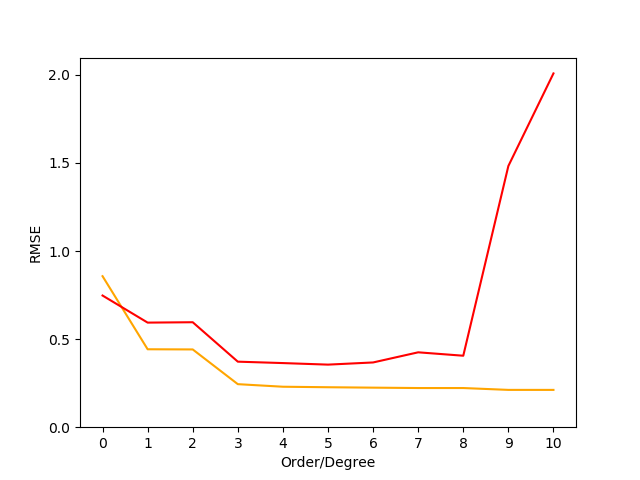
\includegraphics[width=3in]{4.png}
\end{figure} \\
In the figure above, red coorelates to testing data and orange coorelates to training data. The best degree polynomial would be one in the range of the third degree to the seventh degree. Anything less than that exhibits signs of underfitting as RMSE for both training and test data are relatively high. Anything higher than the seventh degree exhibits signs of overfitting as the RSME for the test data spikes sharply (while the RSME for the training data remains low).
}
\end{enumerate}
\end{document}